\documentclass[11pt]{article}
%\documentclass[11pt]{amsart}
\usepackage{graphicx}
\usepackage{epstopdf}
\usepackage{amsmath}
\usepackage[authoryear]{natbib}
\bibliographystyle{chicago}
\usepackage{soul}
\usepackage{verbatim} %multiline commenting
\usepackage{framed} %box paragraphs
\usepackage[font={footnotesize,bf},labelfont=bf]{caption} % font for the figure captions
%\usepackage[showframe]{geometry}
\usepackage{geometry}
\usepackage{layout}

%\documentclass[11pt]{amsart}
%\usepackage{graphicx}
%\usepackage{epstopdf}
%\usepackage{amsmath}
%\usepackage[authoryear]{natbib}
%\bibliographystyle{chicago}
%\usepackage{soul}
%\usepackage{verbatim} %multiline commenting
%\usepackage{framed} %box paragraphs
%\usepackage[font={footnotesize,bf},labelfont=bf]{caption} % font for the figure captions
%%\usepackage[showframe]{geometry}
%\usepackage{geometry}
%%\geometry{letterpaper}
%%\textwidth =6.5in
%%\marginparwidth = 0pt
%%\marginparsep=0pt
%%\oddsidemargin = 0pt
%%\hoffset = 0in
%%\topmargin = 0in
%%\headheight = 0in
%%\headsep = 0pt
%%\footskip=.5in
%%\textheight=8.5in
%%\usepackage{layout}


\usepackage{listings}
\usepackage{textcomp}
\lstset{language=Python,breaklines=true,upquote=true,commentstyle=\normalsize,frame=single}
\DeclareGraphicsRule{.tif}{png}{.png}{`convert #1 `dirname #1`/`basename #1 .tif`.png}

\title{Phase-resolved Wave Prediction from a SWIFT Buoy Array}
\author{Michael Schwendeman}
\date{30 April, 2017}  

\begin{document}

\maketitle
\section{Introduction}
This project is motivated by a long-standing problem in wave-energy generation.  It is known that wave energy converters (WECs) can produce significant gains in efficiency by using advanced control techniques \citep{Li:2012}.  However, such techniques often require advanced knowledge of the incoming waves \citep[see, for example,][]{Hals:2011}.  In the ideal case, the system is given an exact trace of the future wave excitation force.  As this is a difficult problem, most WECs are tuned instead based only on the average 30-minute bulk wave parameters. 

The goal of this project is to provide a useful prediction of the incident waves on a WEC, using an array of networked buoys.  By useful we mean that when coupled with advanced control techniques, the wave prediction improves upon the WEC performance over just using average wave parameters.
A related question, which may have widespread scientific applicability, is whether we can construct a realistic approximation of the sea surface from the sparse buoy array.

This report documents the progress made so far on these questions.  It is broken into three sections.  Section 2 outlines the integration of the SBG Ellipse IMU into the newest version (``v4") SWIFT buoys, and describes the Python program for receiving data in real-time using TCP-IP sockets and an RF ethernet bridge.  Section 3 details the development of a phase-resolved wave prediction algorithm using linear sea surface simulations of directional spectra.  Section 4 shows a preliminary evaluation of the phase-resolved algorithm using real data obtained from a research cruise off of Southern California.  As this is very much a work in progress, each section includes several recommendations and ideas for future work, which are together summarized at the end of the report.
%\subsection{}

\section{SBG and Ethernet Bridge Integration}

\subsection{System Overview}

A schematic of the buoy array approach to wave prediction is shown in Figure \ref{fig:WavePredictionSchematic}.  One of the major design considerations of the new SWIFT (surface wave instrument float with tracking) v4 drifters was their use in the wave prediction problem.  As in the version 3 SWIFTs, the SWIFT v4 is built around a Sutron Xpert microprocessor and data logger.  The Xpert has a 32-bit processor, supports SD memory, and has multiple serial and ethernet ports.  The Xpert logs the raw measurements from the SWIFT sensor payload, and performs onboard processing of certain data products.  These products are then transmitted over Iridium satellite communication to a server on land once per hour.

\begin{figure}[t]
    \centering
    \noindent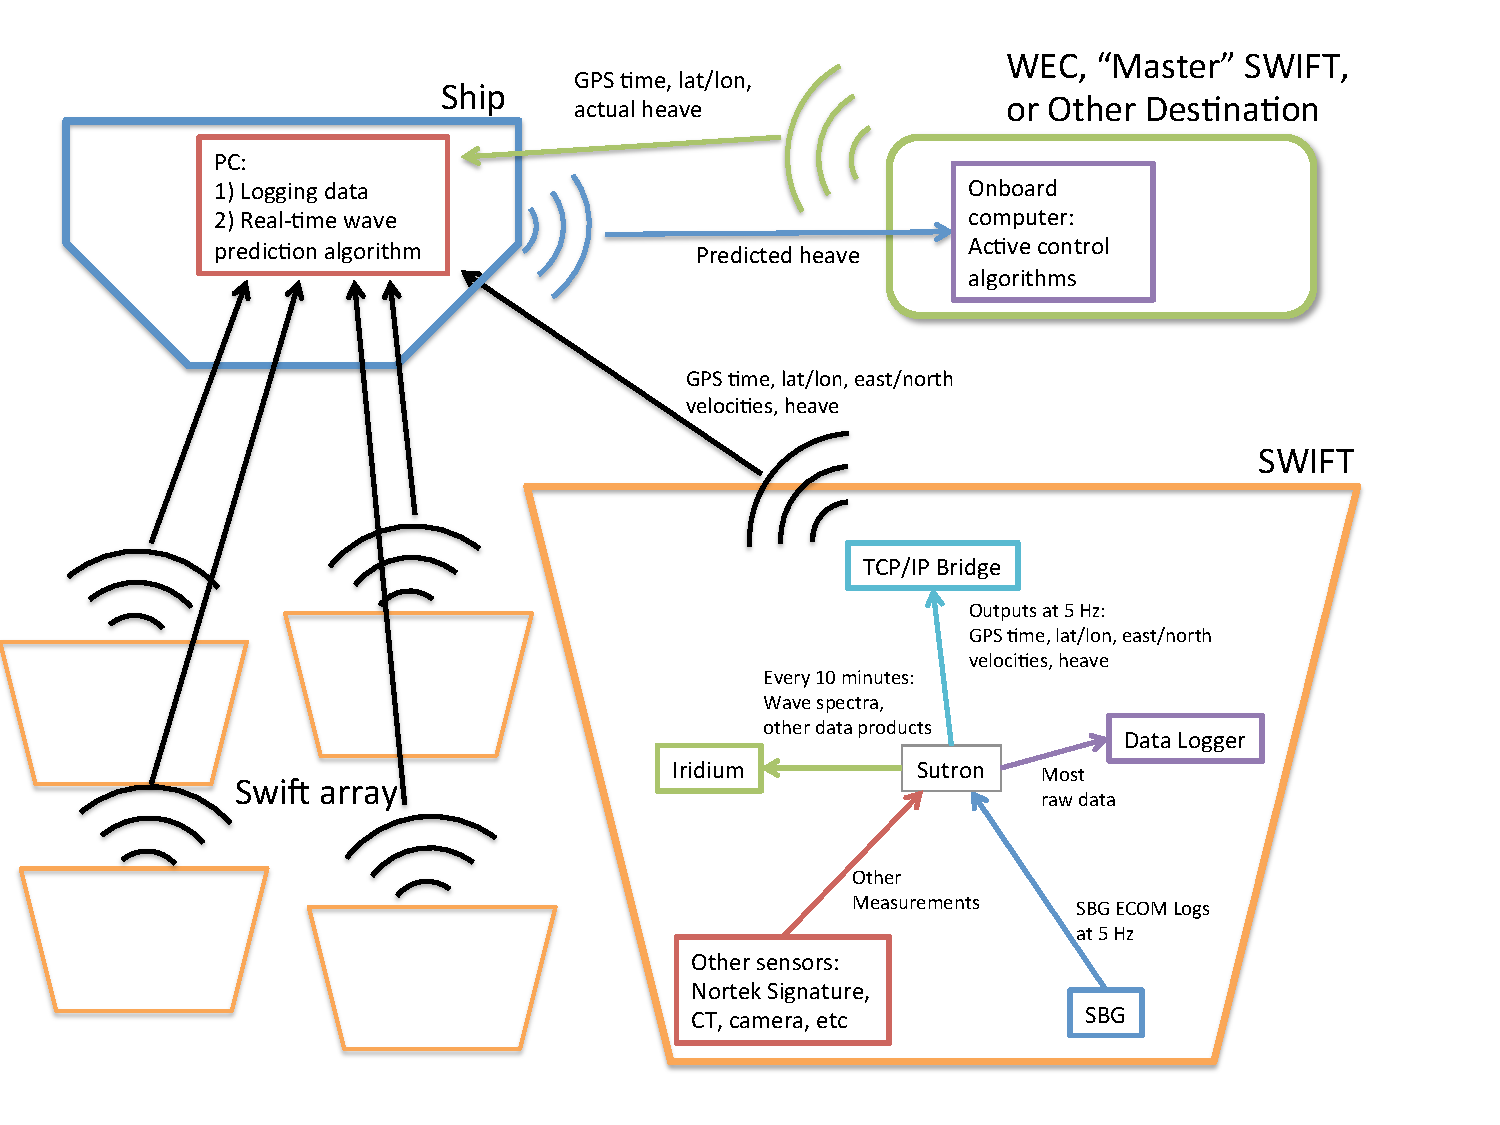
\includegraphics[width=5.5in]{WavePredictionSchematic.pdf}\\
   \vspace{-0in}\caption{Schematic showing the main components of the SWIFT buoy array and wave prediction architecture.}\label{fig:WavePredictionSchematic}
\end{figure}

The form factor of v4 buoys is significantly different than that of the previous SWIFTs, to accommodate the down-looking Nortek Signature 5-beam ADCP.  The v4 buoys no longer have the tall spar-type shape of the previous SWIFTs, which makes them slightly more susceptible to tipping motions.  Ballast was added to the buoy hulls below the water line to limit this effect, and drogues have been experimented with as well.  

For the purposes of this project, the most important change in the SWIFT architecture is the transition from a MicroStrain inertial package to one made by SBG Systems.  The SBG Ellipse-N is a miniature, high-performance MEMS based inertial system with an industrial GNSS receiver.  The Ellipse-N inertial motion unit (IMU) features three-axis gyroscopes, accelerometers, and magnetometers.  It also runs a real-time Extended Kalman Filter (EKF) for data fusion of its IMU and GPS measurements.  In combining the IMU and GPS data streams, the EKF uses the advantages of each measurement to produce a better position and orientation solution than from either measurement alone.  

The most critical measurement of the SWIFTs for real-time wave prediction is the buoy vertical position, or heave.  This is a difficult measurement because it requires two integrations of the inertial accelerometer signal, which leads to drift in the position.  At the same time, the accuracy of the GPS measurements is much worse in the vertical direction than horizontal.  To solve this problem, SBG have developed an advanced high pass filter specifically intended for estimating heave in real-time for marine purposes.  The filter is designed to limit phase and gain errors in wave motions with periods shorter than 15 seconds.

\subsection{SBG Ellipse Configuration and Magnetometer Calibration}
The SBG Ellipse-N is configured and calibrated using the sbgCenter application, which requires the device to be plugged in through serial or usb connectors.  sbgCenter allows you to set the output logs, connection settings, device orientation, lever arms, and aiding sensors (such as GPS).  The device saves its most recent configuration, so this step does not need to be repeated for each deployment.  Configuration settings are also saved and can be loaded from a file. See the dropbox SBG Systems folder in the SWIFT\_v4.x directory for the most up-to-date configuration.

One additional step is needed to ensure accurate measurements from the Ellipse, which is calibration of the internal magnetometer.  This is necessary because although the Ellipse comes calibrated from the factory, placing the Ellipse in the SWIFT puts it near components which may distort the magnetic field.  In this way the uncalibrated Ellipse heading measurement may be off by tens of degrees, which would seriously effect the accuracy of many of the necessary data products.  The calibration procedure is described in the Ellipse Hard \& Soft Iron Calibration Manual.  Unfortunately, the calibration uses the sbgCenter application, which requires the device to be plugged in to the computer.  Thus, the SWIFT cannot be fully sealed, which leaves open the possibility for small errors.  Caveats aside, the calibration procedure appears to bring the average heading error down from roughly 5\% or more to 1-2\%.

\subsection{Receiving SBG Data Over Ethernet Bridge}
The SBG Ellipse-N data is stored and transmitted as messages using the "sbgECom" binary protocol, as described in the Firmware Reference Manual.  The binary messages are logged to a file by the Xpert processor, and also transmitted asynchronously over a TCP/IP socket bridge.  The TCP/IP signal is then wirelessly transmitted over RF radio (900 MHz) via the Digi XPress Ethernet Bridge.  The XPress Ethernet Bridge has a stated range of 2-15 miles depending on the antenna used, and a data rate of 1.5 Mbps.  In Figure \ref{fig:WavePredictionSchematic}, the data from the SWIFT array and WEC (or other target point) are sent to a shipboard PC, where the prediction algorithm is run and returned to the WEC for active controls.  Alternatively, it may be preferable to have the algorithm running in an embedded system onboard the WEC.  

To stream data over the ethernet bridge to the PC, first follow the directions in the file Xpert\_EthernetBridge\_setup.txt.  This sets the IP addresses, Mac addresses, ports, etc. for both sides of the bridge --- namely the shipboard PC and Xpert microprocessor on the SWIFT.  To check that the Ethernet Bridge is setup properly, simply open a browser and navigate to the device IP address, where a screen will show statistics of the connection and device information, as shown in Figure \ref{fig:XpressBrowserInterface}.

\begin{figure}[t]
    \centering
    \noindent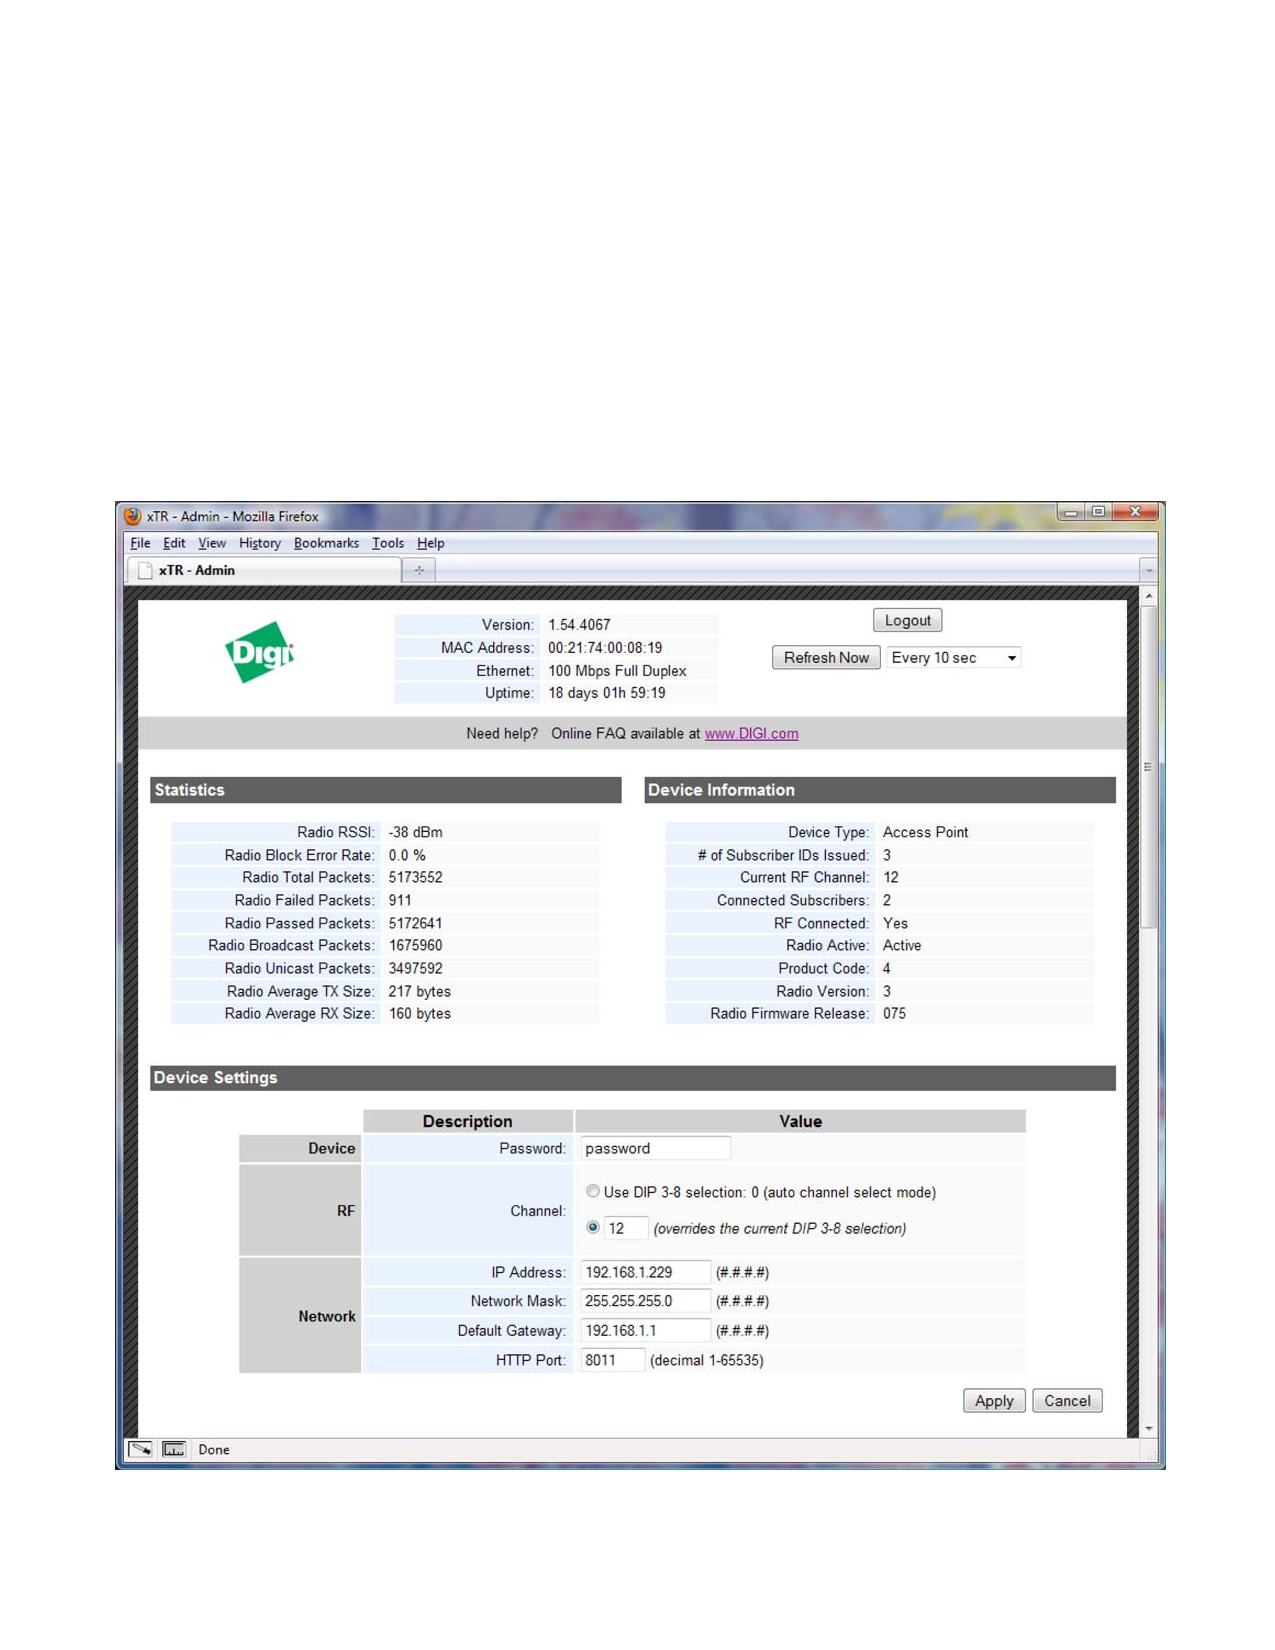
\includegraphics[width=5.5in]{XpressBrowserInterface.pdf}\\
   \vspace{-0in}\caption{Example of the Digi Xpress Ethernet Bridge browser interface.}\label{fig:XpressBrowserInterface}
\end{figure}


The software for receiving data from the SWIFTs and decoding the SBG binary messages is written in Python and contained in two files, which are outlined below. The file \texttt{readAndDecodeFromEthernetBridge.py} is a script which, when run from the PC, opens a TCP/IP socket, listens for incoming connections, and accepts data as available.  In this way, the PC acts as a server, in that it does not query for data, but accepts the data asynchronously.  The TCP/IP functionality is accessed through the Python socket module, which is available on all modern Unix, Windows, and MacOS platforms.  

As the data streams in, a series of if-statements check for the sync bytes that indicate the beginning of an sbgECom message, as detailed in the Ellipse Firmware Reference Manual.  When such a message is detected, the script calls a function \texttt{parseSbgMessage} which further decodes the binary data.  The parsing functions are accessed through the \texttt{sbgMessageParse} module contained in the file \texttt{sbgMessageParse.py}.  The function \texttt{\\parseSbgMessage} was written such that it can read binary data from a socket connection, as indicated above, or from a previously saved raw binary file.  In addition, it can print decoded data in ascii format to a file or to stdout.  The default behavior is to read the data from a socket connection and not print the output.

 A key piece of the parsing is the dictionary variable \texttt{sbgMessages}.  The \texttt{sbgMessages} dictionary contains all the information from the Firmware Reference Manual on the message ID, message name, message length (in bytes), field names, and field types (e.g. 8-bit unsigned integer, double float, etc.). For example, take the first entry:
 \begin{lstlisting}
sbgMessages = {b'\x01': {'name':'Status','intLength':22,'binLength': b'\x16\x00','unpackString':'<LHHLLLH','fields':('time_stamp','general_status','reserved1','com_status','aiding_status','reserved2','reserved3'),...
\end{lstlisting}
 This indicates that messages with \texttt{msgID}=1 (b`\textbackslash x01' in Python binary syntax) has name `Status,' length of 22 bytes (b`\textbackslash x16\textbackslash x00' in binary), and fields \texttt{`time\_stamp'} (unsigned 32 bit integer, or ``L"), \texttt{`general\_status'} (unsigned 16 bit integer, or ``H"), etc.  All of this information is taken from the Ellipse Firmware Reference Manual.  This format makes it easy to add entries to the \texttt{sbgMessages} dictionary if new SBG messages are required at a later time. 
  
The function \texttt{parseSbgData} is called by the wrapper function \texttt{parseSbgMessage}, and is responsible for actually translating the binary messages into a usable Python data structure.  The code is quite compact:
 \begin{lstlisting}
### Function for parsing binary SBG messages into dictionaries     
def parseSbgData(msgID,binData):
    parsedData = struct.unpack(sbgMessages[msgID]['unpackString'],binData)
    dataStruct = OrderedDict(zip(sbgMessages[msgID]['fields'],parsedData))
    return dataStruct
\end{lstlisting}
 It uses the unpack function of the struct library to translate the message bytes into a tuple of integers and floats, as defined in the \texttt{unpackString} of the \texttt{sbgMessages} dictionary. Then, it puts those values into an ordered dictionary with the field names for that message type, also defined in the \texttt{sbgMessages} dictionary.  This \texttt{dataStruct} ordered dictionary is the final result of the parsing and is returned and/or printed.  The Python ordered dictionary works just like a regular dictionary except that when printed, the fields are always in order (i.e. with \texttt{time\_stamp} always printing first).

 
Finally, it should be noted that streaming and decoding of the SBG data could alternatively have been performed using C++.  Specifically, C comes with its own sockets library, and SBG provides an API, written in C++, which can decode the binary messages.  Python was used as it provided a more user-friendly approach, more online support, and easier debugging.  Additionally, a similar decoder was written in Matlab (function \texttt{sbgBinaryToMatlab.m} and script \texttt{sbgBinaryToMatlab\_Batch.m}) for use with logged binary files.  For example, these Matlab functions are used to decode the binary data for testing the prediction algorithm in Section 4.

\subsection{Future Work}

Some additional work is needed to operationalize the above procedure.  Notably, the Ethernet Bridge has not been tested in long range outside, and has not been installed permanently on the SWIFT hulls.  The system has been tested in the laboratory however, and works well to capture and decode SBG data from a single SWIFT over the Ethernet Bridge.  

The \texttt{readAndDecodeFromEthernetBridge.py} program needs to be written to accommodate multiple SWIFTs.  This may be slightly tricky, as the current script is quite linear.  It seems that rather than wait for one connection, it could be modified to wait for four (or as many SWIFTs are in use).  Meanwhile, in the \texttt{while True} loop, it could receive bytes from each connection and parse them one after another.  However, this flow has not yet been tested.  Alternatively, a more complex program would make use of the asynchronous processing modules available in Python, such as \texttt{asynchio}.

A helpful feature of the system is that data is saved in a buffer until the PC is ready to receive the data, so bytes are not lost.  Along the same lines, one feature that has not been implemented is a cyclic redundancy check (CRC), which can be used to look for dropped bytes in the data.  The outline of such a function is given in the SBG Firmware Reference Manual.

With the above modifications, the system will be able to run on a shipboard PC or embedded system onboard a WEC, allowing it to receive, parse, and save timestamped location and heave data from multiple SWIFTs over the RF Ethernet Bridge.  At which point, the next step will be to implement an algorithm which takes in that data, and outputs a prediction (in real time) of the incoming waves to the WEC.  The next sections outline the progress being made in the development of such an algorithm.

\section{Linear Simulations and Least Squares Prediction Algorithm}

\subsection{Least Squares Prediction Algorithm}

Our goal is to develop an algorithm which, given a sparse array of wave measurements, can predict (in some way) the waves that will pass a different point at a later time.  \citet{Connell:2015} describe one such algorithm, which is based on a least squares fit of the measurements to different wave components, which are then propagated forward in time by assuming linear dispersion.  Given enough observations and minimal nonlinearity, this method yields a highly accurate time-domain, phase-resolved forecast of the approaching waves.  The  \citet{Connell:2015} paper is written around the use of a coherent Doppler radar for making the wave observations.  The advantage of radar over a sparse buoy is in the much larger number of observations, with much better spatial coverage.  One downside is that the radar can only estimate the radial wave orbital velocity, rather than surface elevation, which slightly complicates the analysis.  

The algorithm is based around the representation of the sea surface as a sum of individual wave components, as in
\begin{eqnarray} \label{eq:WaveComponents}
\eta(\mathbf{x},t) = \Re \left(\sum_{n=1}^{N}A_n \exp(i(\mathbf{x}\cdot\mathbf{k}_n-\omega_nt))\right)
\end{eqnarray}
where $A_n$, $\mathbf{k}_n$, and $\omega_n$ are the amplitude, wavenumber, and frequency of each component.  Assuming linear dispersion, then gives
\begin{eqnarray}
\omega = \sqrt{gk}
\end{eqnarray}
where $g$ is gravitational acceleration and 
\begin{eqnarray}
k=\sqrt{k_x^2+k_y^2}.  
\end{eqnarray}
This equation can be expressed in matrix form as
\begin{eqnarray}
\mathbf{\eta} = \mathbf{P}\mathbf{A}
\end{eqnarray}
where $\mathbf{P}$ is an $N\times M$ matrix with elements
\begin{eqnarray}
P_{n,m} = \exp(i(\mathbf{x}_m\cdot\mathbf{k}_n-\omega_n t_m)),
\end{eqnarray}
called the propagator matrix.  $\mathbf{\eta}$ is an $M\times1$ vector of observations, and $\mathbf{A}$ is an $N\times1$ vector of unknown wave amplitudes.  If $M>N$, this is an overdetermined system of equations, such that $\mathbf{A}$ can be fit using the linear least squares method.  With the component amplitudes determined in this way, the surface elevation at a desired time and place can be projected using equation \ref{eq:WaveComponents}

The least squares prediction algorithm is implemented in Matlab in the function \texttt{\\leastSquaresWavePropagation.m}.  Below is a slightly simplified version of the code:

\lstset{language=Matlab}
 \begin{lstlisting}
function [z2,zc] = leastSquaresWavePropagation_2D(z1,t1,x1,y1,t2,x2,y2,k,theta,reg_factor)

kx = k*cos(theta');
ky = k*sin(theta');
omega = sqrt(9.8*k)*ones(size(theta'));
P1 = [cos(x1*kx'+y1*ky'-t1*omega'),sin(x1*kx'+y1*ky'-t1*omega')];
A = ridge(z1,P1,reg_factor,0);
P2 = [cos(x2*kx'+y2*ky'-t2*omega'),sin(x2*kx'+y2*ky'-t2*omega')];
z2 = P2*A(2:end);
end
 \end{lstlisting}

Note that the code above shows two slight differences from how the algorithm was first described.  First, is that the wave components are expressed as sines and cosines, rather than the real part of a complex exponential.  In theory, these representations are exactly the same.  However for a reason that is not clear, when complex exponentials are used, the fitted result is off by a factor of two.  This can be readily tested with simple examples using a surface constructed of only a few known components.

The second difference is more conceptually important.  It was found often that using a pure least squares solution led to overfitting, thus it was replaced with a regularized least squares method, also called ridge regression.  Overfitting produces large values for the wave component amplitudes, which largely cancel out to reproduce the surface elevation at the observed points, but leads to unphysical surface elevations everywhere else.  Regularization penalizes large values of fitted coefficients,  leading to more realistic results.  However, it also introduces a new parameter, \texttt{reg\_factor}, which controls the degree of penalization.

\subsection{Simulations of Irregular Waves from Directional Spectra}
This problem is aided greatly by the use of synthetic data to test and refine the forecast algorithm.  Thus, the Wave Analysis for Fatigue and Oceanography (WAFO) toolbox is used to produce realistic simulations of irregular ocean waves in three dimensions \citep{WAFO:2000}.  Specifically, the function \texttt{seasim.m} is run, which uses the discrete spectral approximation of \citet{Dietrich:1997} to efficiently simulate 3D surfaces from a given directional wave spectrum.

The wave simulations are carried out in the script \texttt{simulateWaveSurfaceFromDirectional\\Spectrum.m}.  Two inputs are needed from the user.  The first is a source for the directional energy spectrum.  Three examples are given: SWIFT and Datawell Waverider spectra from Station Papa, and CDIP data from San Nicolas Island.  Regardless of the source, the spectrum must be put in WAFO's specified wave spectra structure format, as described in the file \texttt{spec.pdf} in the WAFO toolbox directory.  For example, the wave directions must be in radians and range from $-\pi$ to $\pi$.  Optionally, the script can rotate the directional spectrum such that the peak wave direction (direction energy is propagating from, not to) is aligned with the $+x$ coordinate. Next, the user must define the simulation grid, including spatial and temporal range ($L$ and $T$, in meters and seconds respectively) and resolution ($dx$ and $dt$).  Note that the simulations run slowly and produce large arrays of data when given overly large domains.

The \texttt{seasim} function takes as input the directional spectrum (in WAFO format), and grid dimensions.  It also takes an \texttt{fftdim} parameter, which defines whether the simulation runs a two-dimensional inverse FFT at each timestep (\texttt{fftdim=2}) or a one-dimensional inverse FFT at each spatial grid cell (\texttt{fftdim=1}).  When spectra are made from the simulation data, they appear to match the original (input) spectra better when using the one-dimensional inverse FFT method.  \texttt{seasim} outputs the simulation results as a structure, \texttt{Y}, which has fields \texttt{x, y, t,} and \texttt{Z}.  \texttt{simulateWaveSurfaceFromDirectionalSpectrum.m} finishes by saving the structure \texttt{Y}, and plotting the input directional spectrum and a check of the original frequency spectra with one calculated from the simulated data.  These usually match well, particularly for large simulations, as shown in Figure \ref{fig:FrequencySpectraComparison}.

\begin{figure}[t]
    \centering
    \noindent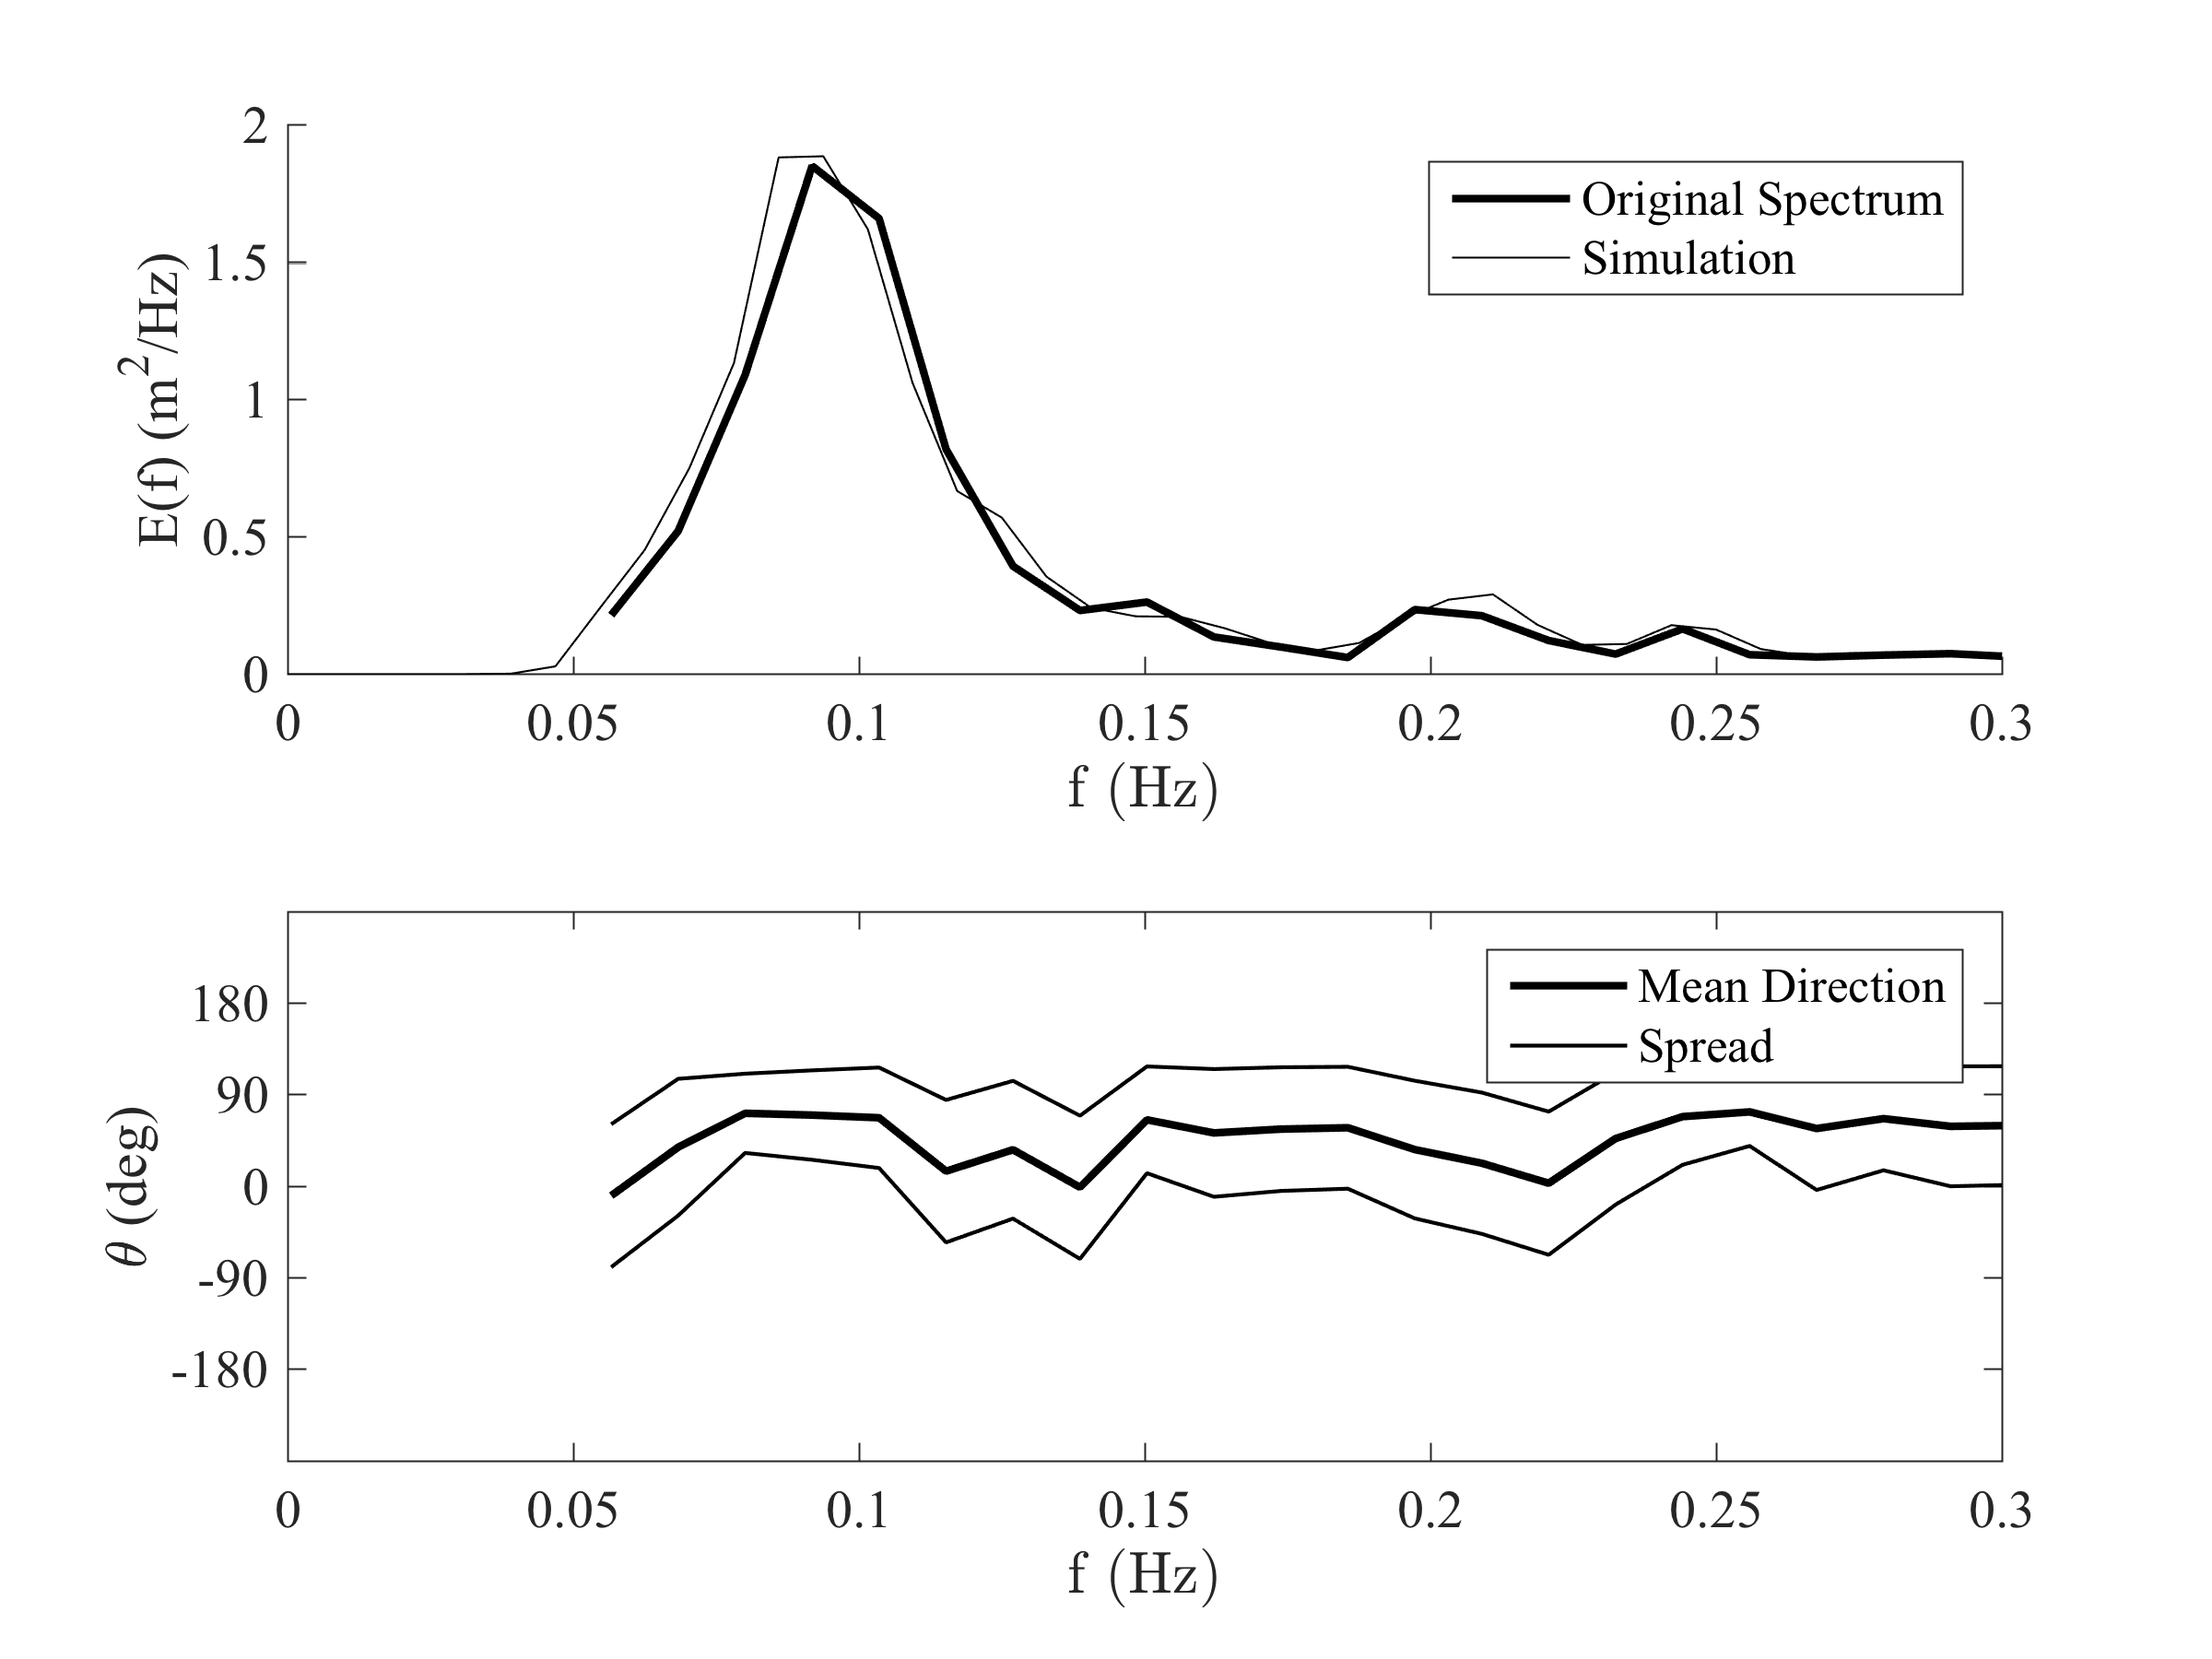
\includegraphics[width=5.5in]{FrequencySpectra.png}\\
   \vspace{-0in}\caption{Example comparison of frequency spectra from \texttt{simulateWaveSurfaceFromDirectional\\Spectrum.m}.  Data from a SWIFT at Station Papa, $L = 500$ m, $T = 300$ s, $dx = 4$ m, $dt = 1$ s.}\label{fig:FrequencySpectraComparison}
\end{figure}

\subsection{Algorithm Performance for Simulated Data}
The synthetic wave data is used to test the validity of the least squares forecast algorithm.  This is done using the script \texttt{testWavePropagationModels.m}, and several helper functions.  Since the simulations are generated using linear dispersion, and the forecast assumes linear dispersion, given enough of the synthetic data the prediction should be almost perfect.  However, we want to test how well the algorithm can predict the waves given only a sparse number of points in the domain, simulating a small array of buoys.  Provided are two examples, \texttt{setBuoyArray\_Circle} and \texttt{setBuoyArray\_Box}, which take in the full synthetic data grid and output \texttt{x, y, } and \texttt{z} vectors of data sampled at ``buoys" in the shape of a circular arc or square box.  An infinite number of other shape options could be tested, but circles and squares seemed a good place to start.

The buoy array shape (including the number of buoys) is just one of the input parameters to the algorithm.  The others are:
\begin{enumerate}
\item{The number of wave components.  These are defined as a vector of wavenumbers, \texttt{k} (in radians), and a vector of directions, \texttt{theta} (also radians).  To solve for the component amplitudes using least squares, an upper limit to the number of wave components is half of the number of observations (because each component has both a sine and cosine term).  Below that limit, more components means better resolution of the wave propagation speed and direction.  However, for many components the solution is less constrained (may be more prone to overfitting) and takes longer to solve.  Good results were found for 30-50 wavenumber components, spaced logarithmically over the energetic range of the energy spectrum, and 10-20 directional components, spaced linearly from -$\pi$ to $\pi$.}
\item{The regularization parameter, \texttt{reg\_factor}, mentioned previously.  This can act in some ways as a ``tuning knob" for the fit, and is not yet well constrained.  Moreover, the optimal regularization factor appears to depend on the number of buoys and the number of wave components.  This makes sense in the context of regularization as a means of preventing overfitting.  Overfitting is less likely with a large number of observations relative to the number of coefficients being fit, thus less regularization (smaller \texttt{reg\_factor}) is needed.}
\item{The observation and prediction time windows. This is needed to simulate the operational aspect of the predictions.  In practice, a window of time of the buoy measurements will be used to predict the waves at the WEC for a length of time later.  Thus, the governing parameters are the length of the observation window (\texttt{T\_meas}), the length of the prediction window (\texttt{T\_pred}), and the time delay between the end of the observation window and the start of the prediction window (\texttt{T\_delay}).  Finally, if the prediction window is shorter than the observation window, some overlap of the observation windows is needed to provide full coverage (\texttt{overlap}). It is expected that the optimal time windowing and delay will be related to the wave conditions (i.e. the dominant wave period and group velocity) and the distance of the buoy array to the WEC.}

\end{enumerate}

The final input is the location of the target point (or points).  In the WEC wave forecast problem, this would be a single point space, which may slightly drift in time depending on the currents, winds, and waves.  A related problem, which may also help troubleshoot the single point forecast, is to construct a gridded surface that approximates the wavefield.  Solutions to these two problems are implemented in separate two functions: \texttt{runLeastSquaresPrediction\_PointComparison.m} and \texttt{runLeastSquaresPrediction\_\\SurfaceReconstruction.m}.  In each case, the inputs include the buoy array observations, wave components, regularization parameter, and time window and delay parameters.  However, whereas in the point prediction case, the target is defined by two $N_t\times1$ vectors of $x$ and $y$ as a function of time, in the surface reconstruction case, the target points are $N_y \times N_x$ matrices of gridded $x$ and $y$ points (static in time).  Note, that it is easily possible to crash Matlab by making the $x$ and $y$ grids too large, for example, the size of the full simulation domain.

The outputs of \texttt{runLeastSquaresPrediction\_PointComparison.m} are the predicted surface elevation at the target point \texttt{z\_pred}, at times \texttt{t\_pred}.  The predictions are of size $N_{t,pred}\times N_{windows}$, where $N_{t,pred} = $ \texttt{T\_pred/dt}, and $N_{windows}$ are the number of prediction windows.  The function also reports the actual measurement at the target point, \texttt{z\_truth}, sampled at the same time as \texttt{z\_pred} for easy comparison.  Meanwhile, 
\texttt{runLeastSquaresPrediction\_SurfaceReconstruction.m} also outputs \texttt{z\_pred} and \texttt{t\_pred}, which are of size $N_{t,pred}\times N_{windows} \times (N_{x}*N_{y})$.  It is assumed that the true surface elevation is not known at each grid point, so no \texttt{z\_truth} array is output.

An example of the simulated forecast is shown below.  The directional spectrum is taken from the CDIP Waverider buoy off San Nicolas Island (CDIP 138), from March 2016.  This data is applicable as it is near the time of year and location of the field experiments described in Section 4.  Furthermore, this example could be considered close to a best case scenario, given a limited number of SWIFTs.  The buoy array is positioned about one wavelength upwave of the target point, with enough spread to determine wave direction.  The wave conditions consist of energetic, long-period swell and very little wind sea, which make for highly coherent wave crests.  And finally, the regularization parameter, time windows, and delay have been tuned for optimal performance.  The relevant parameters are given below.

\lstset{language=Matlab}
 \begin{lstlisting}
arrayShape = 'circle';
% Setup buoy array - Circle
n_theta = 3;
theta_spread = 90; % deg
dir_principal = cell2mat(dspec2char(S_Measured,'Wdir'))*180/pi; % peak direction
theta = linspace(dir_principal-theta_spread/2,dir_principal+theta_spread/2,n_theta)';
circle_radius = [150];

% set time bursts duration/delay etc
T_meas = 30; %sec
T_pred = 10; %sec
T_delay = 5; %sec,
overlap = 0.3; % 1=no overlap, 0.5=50%, etc

% set least squares model values
k = logspace(-3,-1,41)*2*pi;
theta_wavenumber = linspace(-180,180,13)*pi/180;
theta_wavenumber = theta_wavenumber(2:end);
reg_factor = 1e0;
\end{lstlisting}

For these parameters, it takes on average 0.1 seconds to make each 10 second prediction at a single point (note that $dt=1$ second for these simulations, so this would increase for higher fidelity data).  The resulting prediction for a WEC located at the center of the domain is shown in Figure \ref{fig:SimulationPointComparison}.  The top panel shows the measured and predicted time series, while the bottom left shows one frame of the simulation and the locations of the array (red) and target (black) points.  Finally, the bottom right panel shows a scatter plot of the measured and predicted time series, and associated $R^2$.  The surface prediction is highly correlated with the ``true" original simulation data, though it tends to systematically underpredict the height of the waves.  This would be improved by adding more SWIFTs, but this provides a good baseline for the  measurements in Section 4.  A similar comparison is shown in Figure \ref{fig:Rendered}, where the buoys and simulation surface have been rendered and animated.  A full movie is available in the documentation folder.

\begin{figure}[t]
    \centering
    \noindent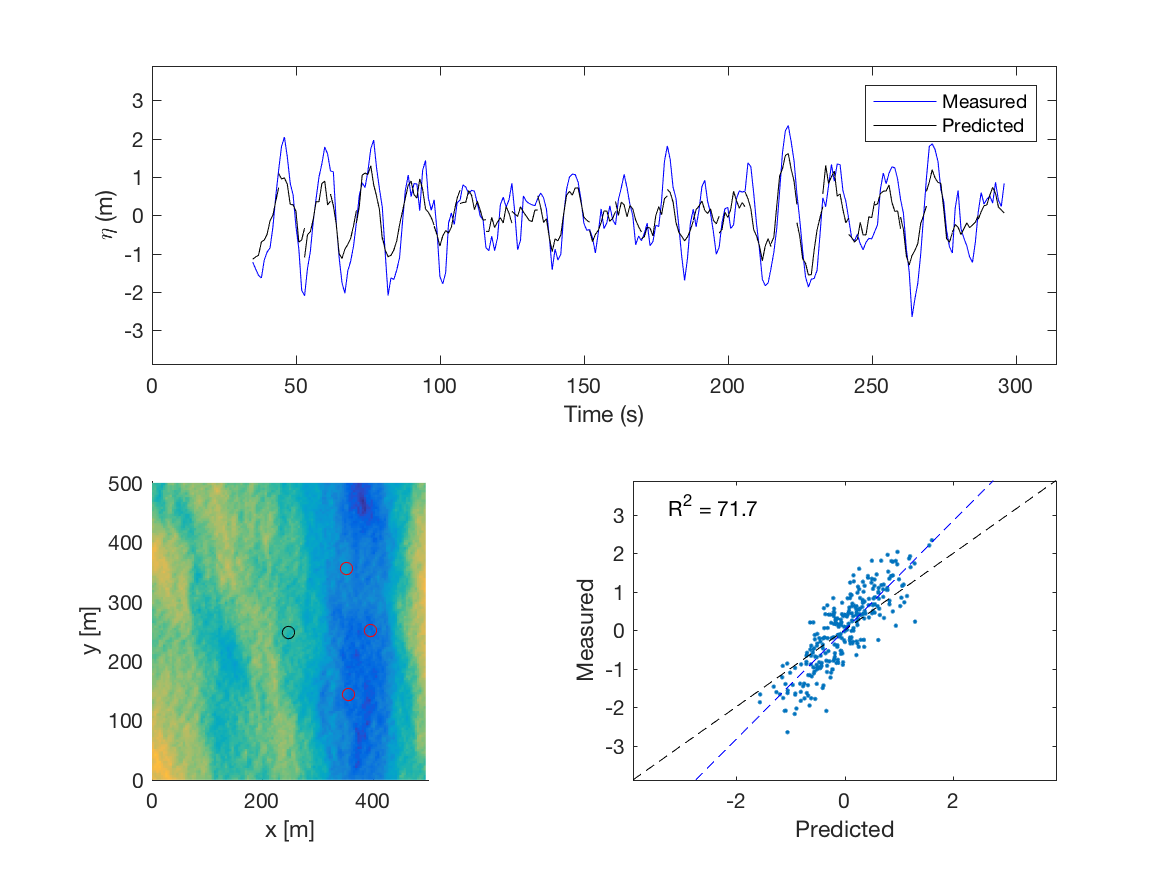
\includegraphics[width=5.5in]{PointPrediction.png}\\
   \vspace{-0in}\caption{Example wave forecast from simulated data.}\label{fig:SimulationPointComparison}
\end{figure}

\begin{figure}[t]
    \centering
    \noindent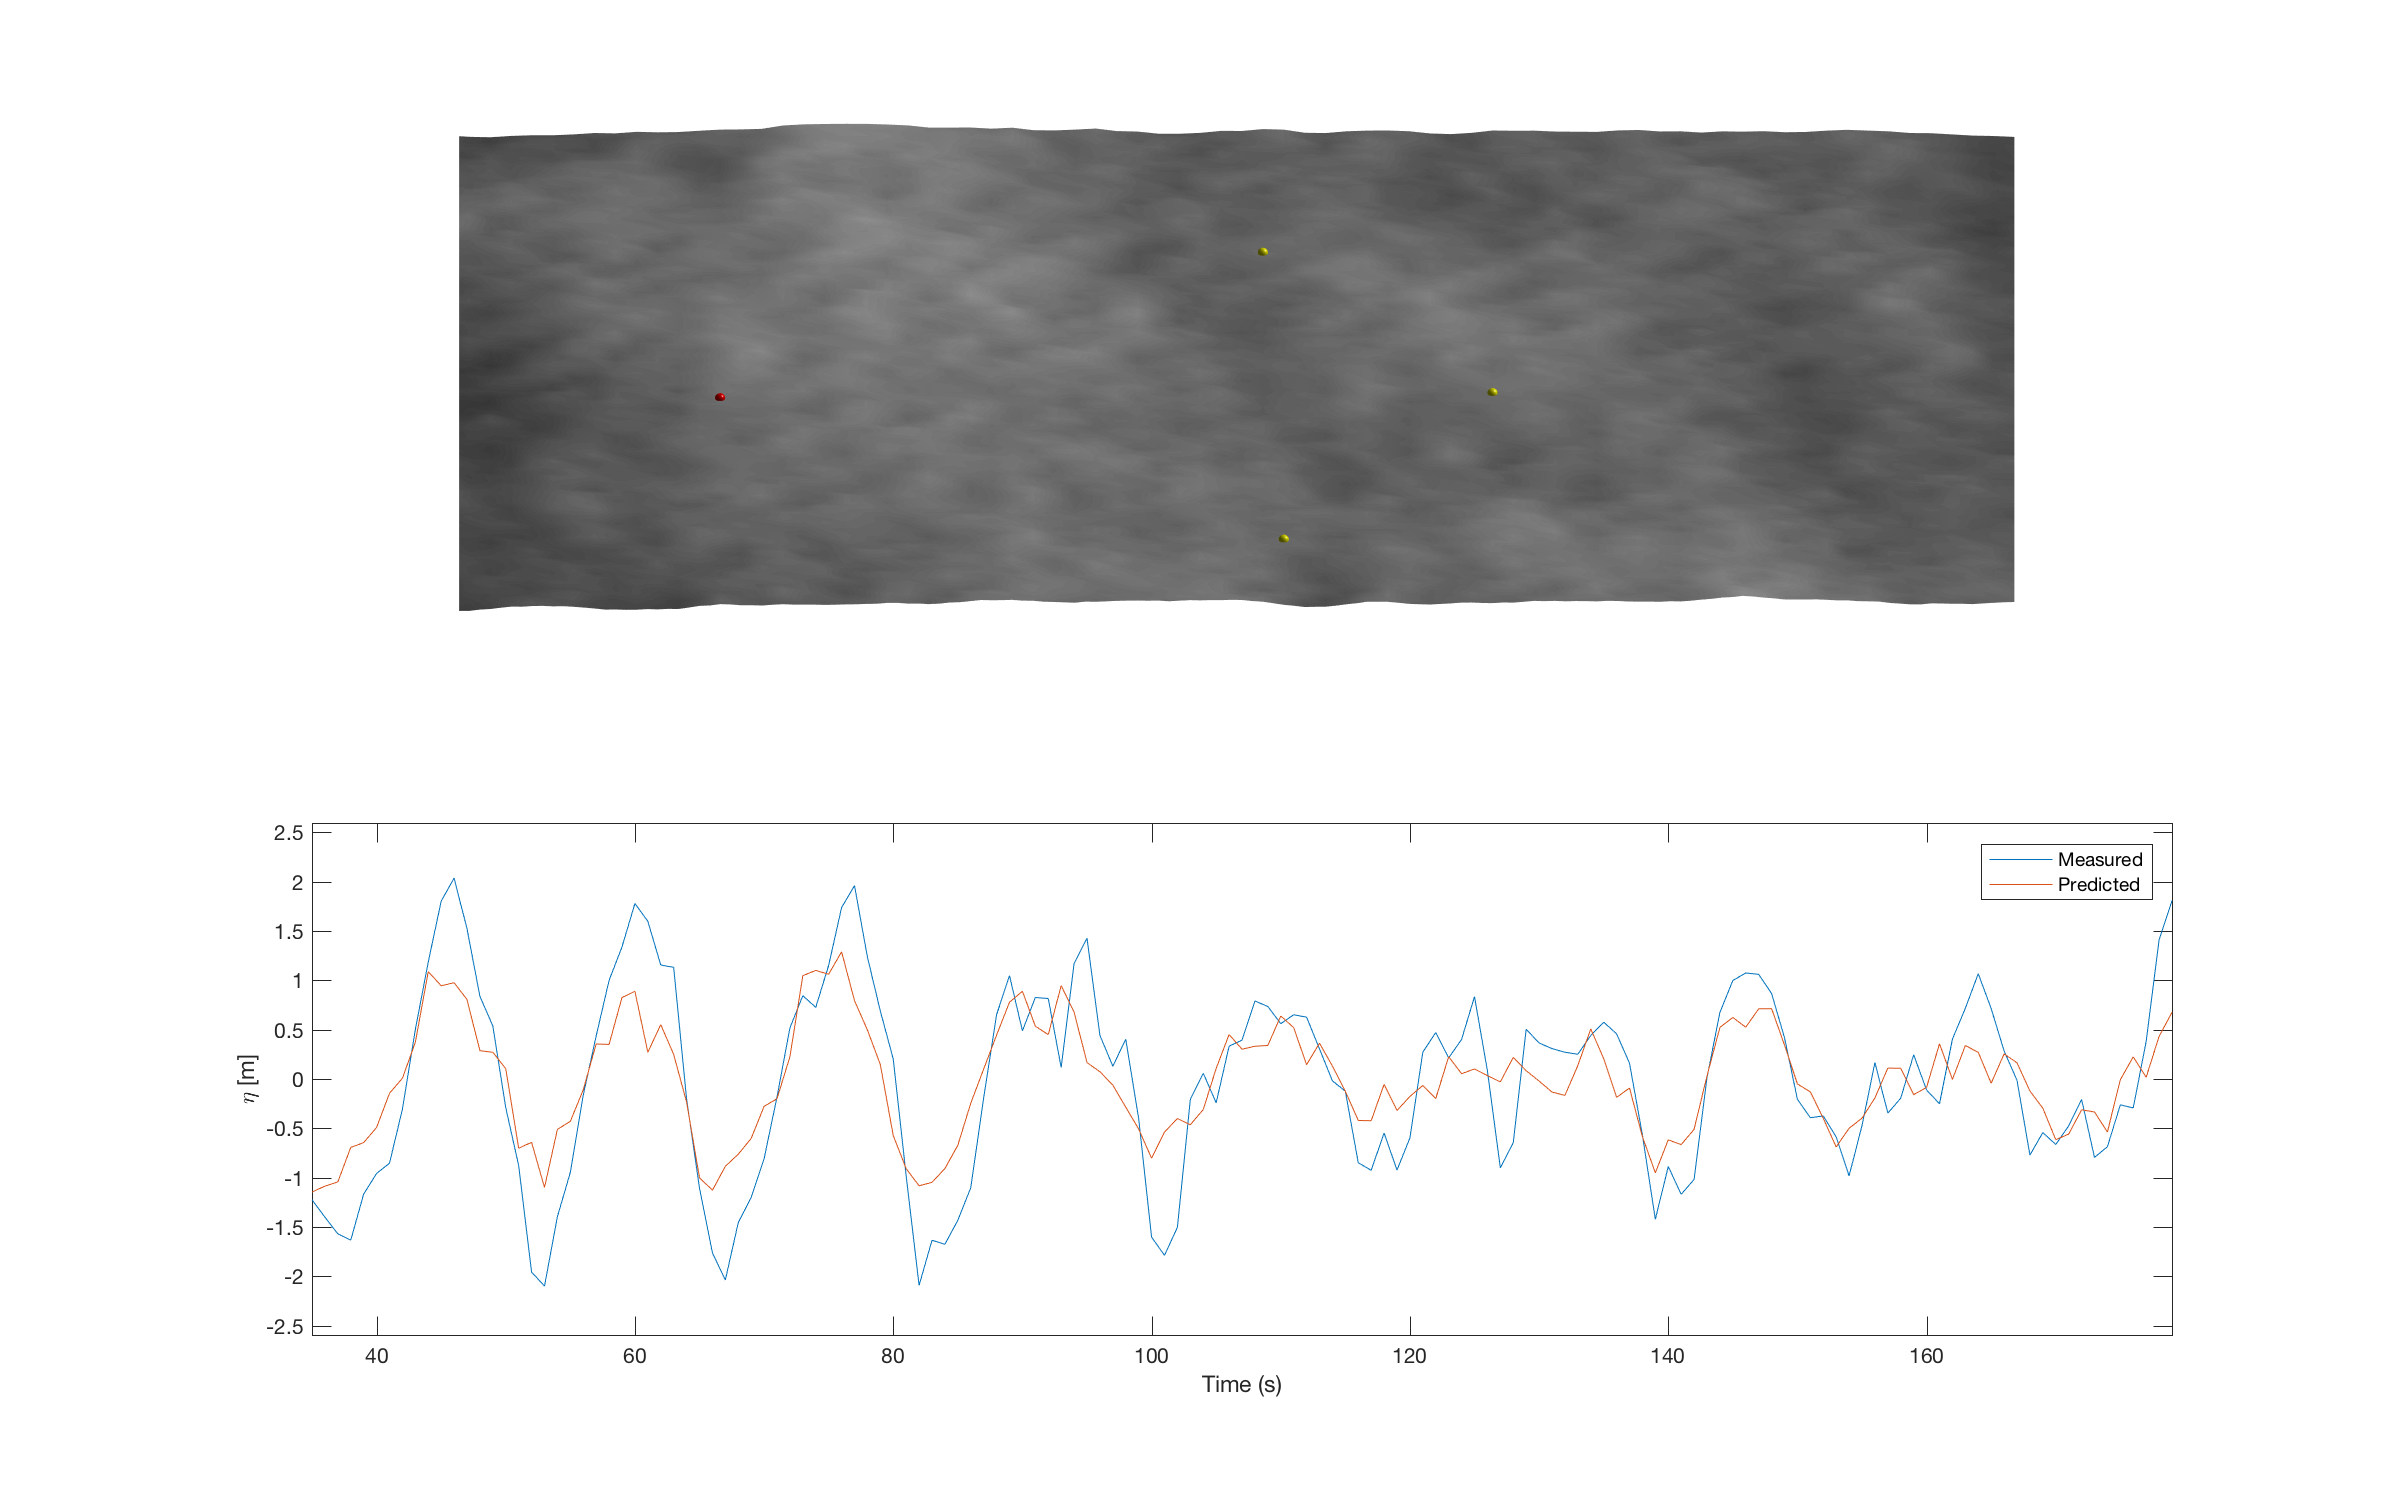
\includegraphics[width=6.5in]{SimulationFrame_145.png}\\
   \vspace{-0in}\caption{Example wave forecast from simulated data (rendered).}\label{fig:Rendered}
\end{figure}

Finally, an example surface reconstruction for the same synthetic data and algorithm parameters is shown in Figure \ref{fig:SurfaceReconstruction}.  Again, a full movie is available in the documentation folder.  As seen in the point-wise comparison, the surface reconstruction movie makes clear that the wave motions are being well captured, with the forecast missing the full extent of the wave peaks and troughs. 

\begin{figure}[t]
    \centering
    \noindent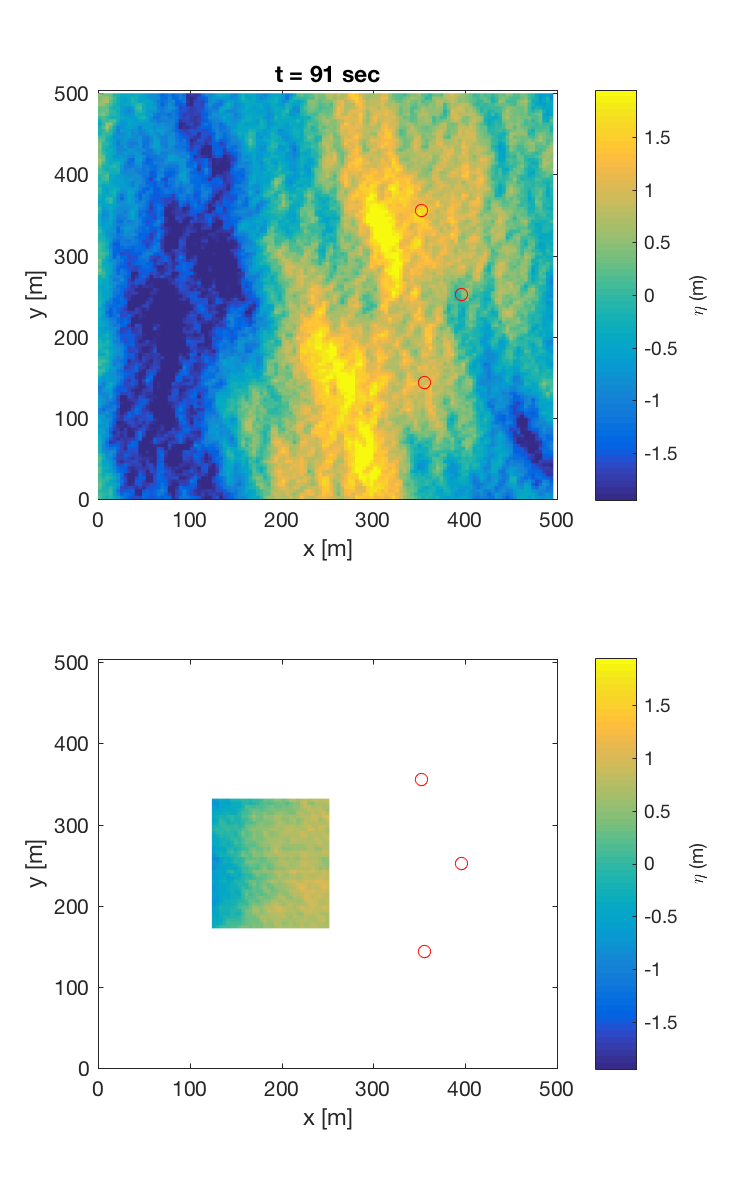
\includegraphics[width=2.5in]{SurfacePrediction_057.png}\\
   \vspace{-0in}\caption{Example surface reconstruction from simulated data.}\label{fig:SurfaceReconstruction}
\end{figure}

\subsection{Future Work}

The simulations prove that the least squares forecast algorithm can work well even with a limited number of buoys, particularly when the conditions are well-suited for the predictions (namely, long-crested, energetic swells with little wind sea).  Moreover, they show that there is significant sensitivity based on the spatial location of the buoy array, relative to the wave conditions and the parameters of the least squares fit.  Clearly, there are many questions that the synthetic data cannot address, such as the complicating factor of nonlinearity.  However, to better inform future field experiments, a systematic analysis of the relationship of the different parameters to the forecast error would be useful.  For example, how does the error scale with the ratio of the buoy array separation to the peak wavelength?  How many buoys are needed, and does it change with different wave conditions?  Perhaps most critical is understanding the time window for making a valid forecast, and how that depends on the other parameters.  There is some work being done on this subject in the laboratory of Dick Yue at MIT, particularly his graduate student Yusheng Qi, although it is as yet unpublished.

These simulations also provide a convenient laboratory for experimenting with the forecast algorithm.  One promising idea for improving the algorithm is to add to the least squares cost function a soft constraint based on the directional wave spectra.  Since on average the wave component amplitudes will match the measured spectra, the best guess of the amplitudes for any one window of data would also match the spectra.  This would amount to providing an individual \texttt{reg\_factor} for each component of the fit, although it is not immediately clear how the spectral values would translate into the cost function values (for example, are they proportional?).  Some care would be needed in implementing this strategy.

\section{Evaluation from SWIFT data}
- Describe LC-DRI experiment.\\
- Example SWIFT wave prediction.\\
- Envelope calculations.\\
- Examine surface reconstruction.\\
- Future work: rolling algorithm with incrementation, use velocity data\\

\section{Summary of Future Work}
The above methodology has shown promise, in simulations and post-processing of real data, for providing a useful wave prediction at a WEC site given the right wave conditions and adequate array placement.  However, there are still several large additions and modifications that must be addressed to prove that it can work operationally in real time.  So far, the operational work and algorithm development have progressed separately, which has been effective and should continue until the necessary improvements have been made on each side.  To summarize, the most pressing needs are:
\begin{itemize}
\item{Testing of the communication of real-time SWIFT array data over the Ethernet Bridge in open water, and logging on the WEC embedded computer using the Python code.  Also, modification of the Python code to handle incoming data from multiple SWIFTs.}
\item{Algorithm improvements, including implementation of a rolling estimator constrained by the previous 30-minute directional spectra.  These would help against over-fitting to wave components with high frequencies and unrealistic wave directions, and would smooth discontinuities between prediction windows.  The use of $u$ and $v$ velocities from GPS may prove more accurate in the field data}.
\item{A systematic error analysis that will help to determine the parameters of the prediction algorithm in an operational setting.  For example, how many buoys are needed and how close together must they be for a given set of wave conditions?  Or, how to choose the time window and delay of the prediction based on the waves and the distance between array and target?}
\end{itemize}
Finally, the results of these experiments need to be discussed with the experts in WEC dynamics and controls, to better decide on what outputs would be useful on their end.  It is likely that even an imperfect phase-resolved wave prediction would be an improvement over the current state of the art, which uses only the average wave statistics.

\bibliography{/Users/mike/Documents/UW/Research/Reading/allReferences}

\end{document}  